\chapter{MCollective}
\label{comun:mcollective}


MCollective es un sistema de despliegue de servidores y de sistemas de ejecución de trabajos en paralelo. Su función principal dentro del ámbito de la administración de sistemas es la ejecución de una acción sobre un conjunto de servidores. Para lograr esto, MCollective se apoya en un \emph{middleware} que proporciona un servicio publicador-suscriptor. En este tipo de programas, las publicaciones y suscripciones suelen implementarse mediante el paso de mensajes asíncrono. Una de las posibilidades que se pueden usar con MCollective es RabbitMQ (Apéndice \ref{comun:rabbitmq}), que implementa el estándar de paso de mensajes AMQP (Advanced Message Queuing Protocol).

Dentro de la arquitectura MCollective, los componentes más importantes son:
\begin{itemize}
\item Cliente: Indica las órdenes a ejecutar.
\item \emph{Middleware}: Lleva las órdenes del cliente a los servidores.
\item Servidor: Cumple las órdenes que le son enviadas.
\end{itemize}

El funcionamiento habitual de MCollective consiste en el lanzamiento de una orden desde el cliente que es transmitida a todos los servidores (\emph{broadcast}) y éstos la llevan a cabo. En la figura \ref{figure:arquitectura-mcollective} se puede apreciar como la instrucción emitida por el cliente llega al corredor de mensajes (\emph{broker}) y éste lo hace llegar a los servidores para que la cumplan.

\begin{figure} [!htbp]
  \centering
  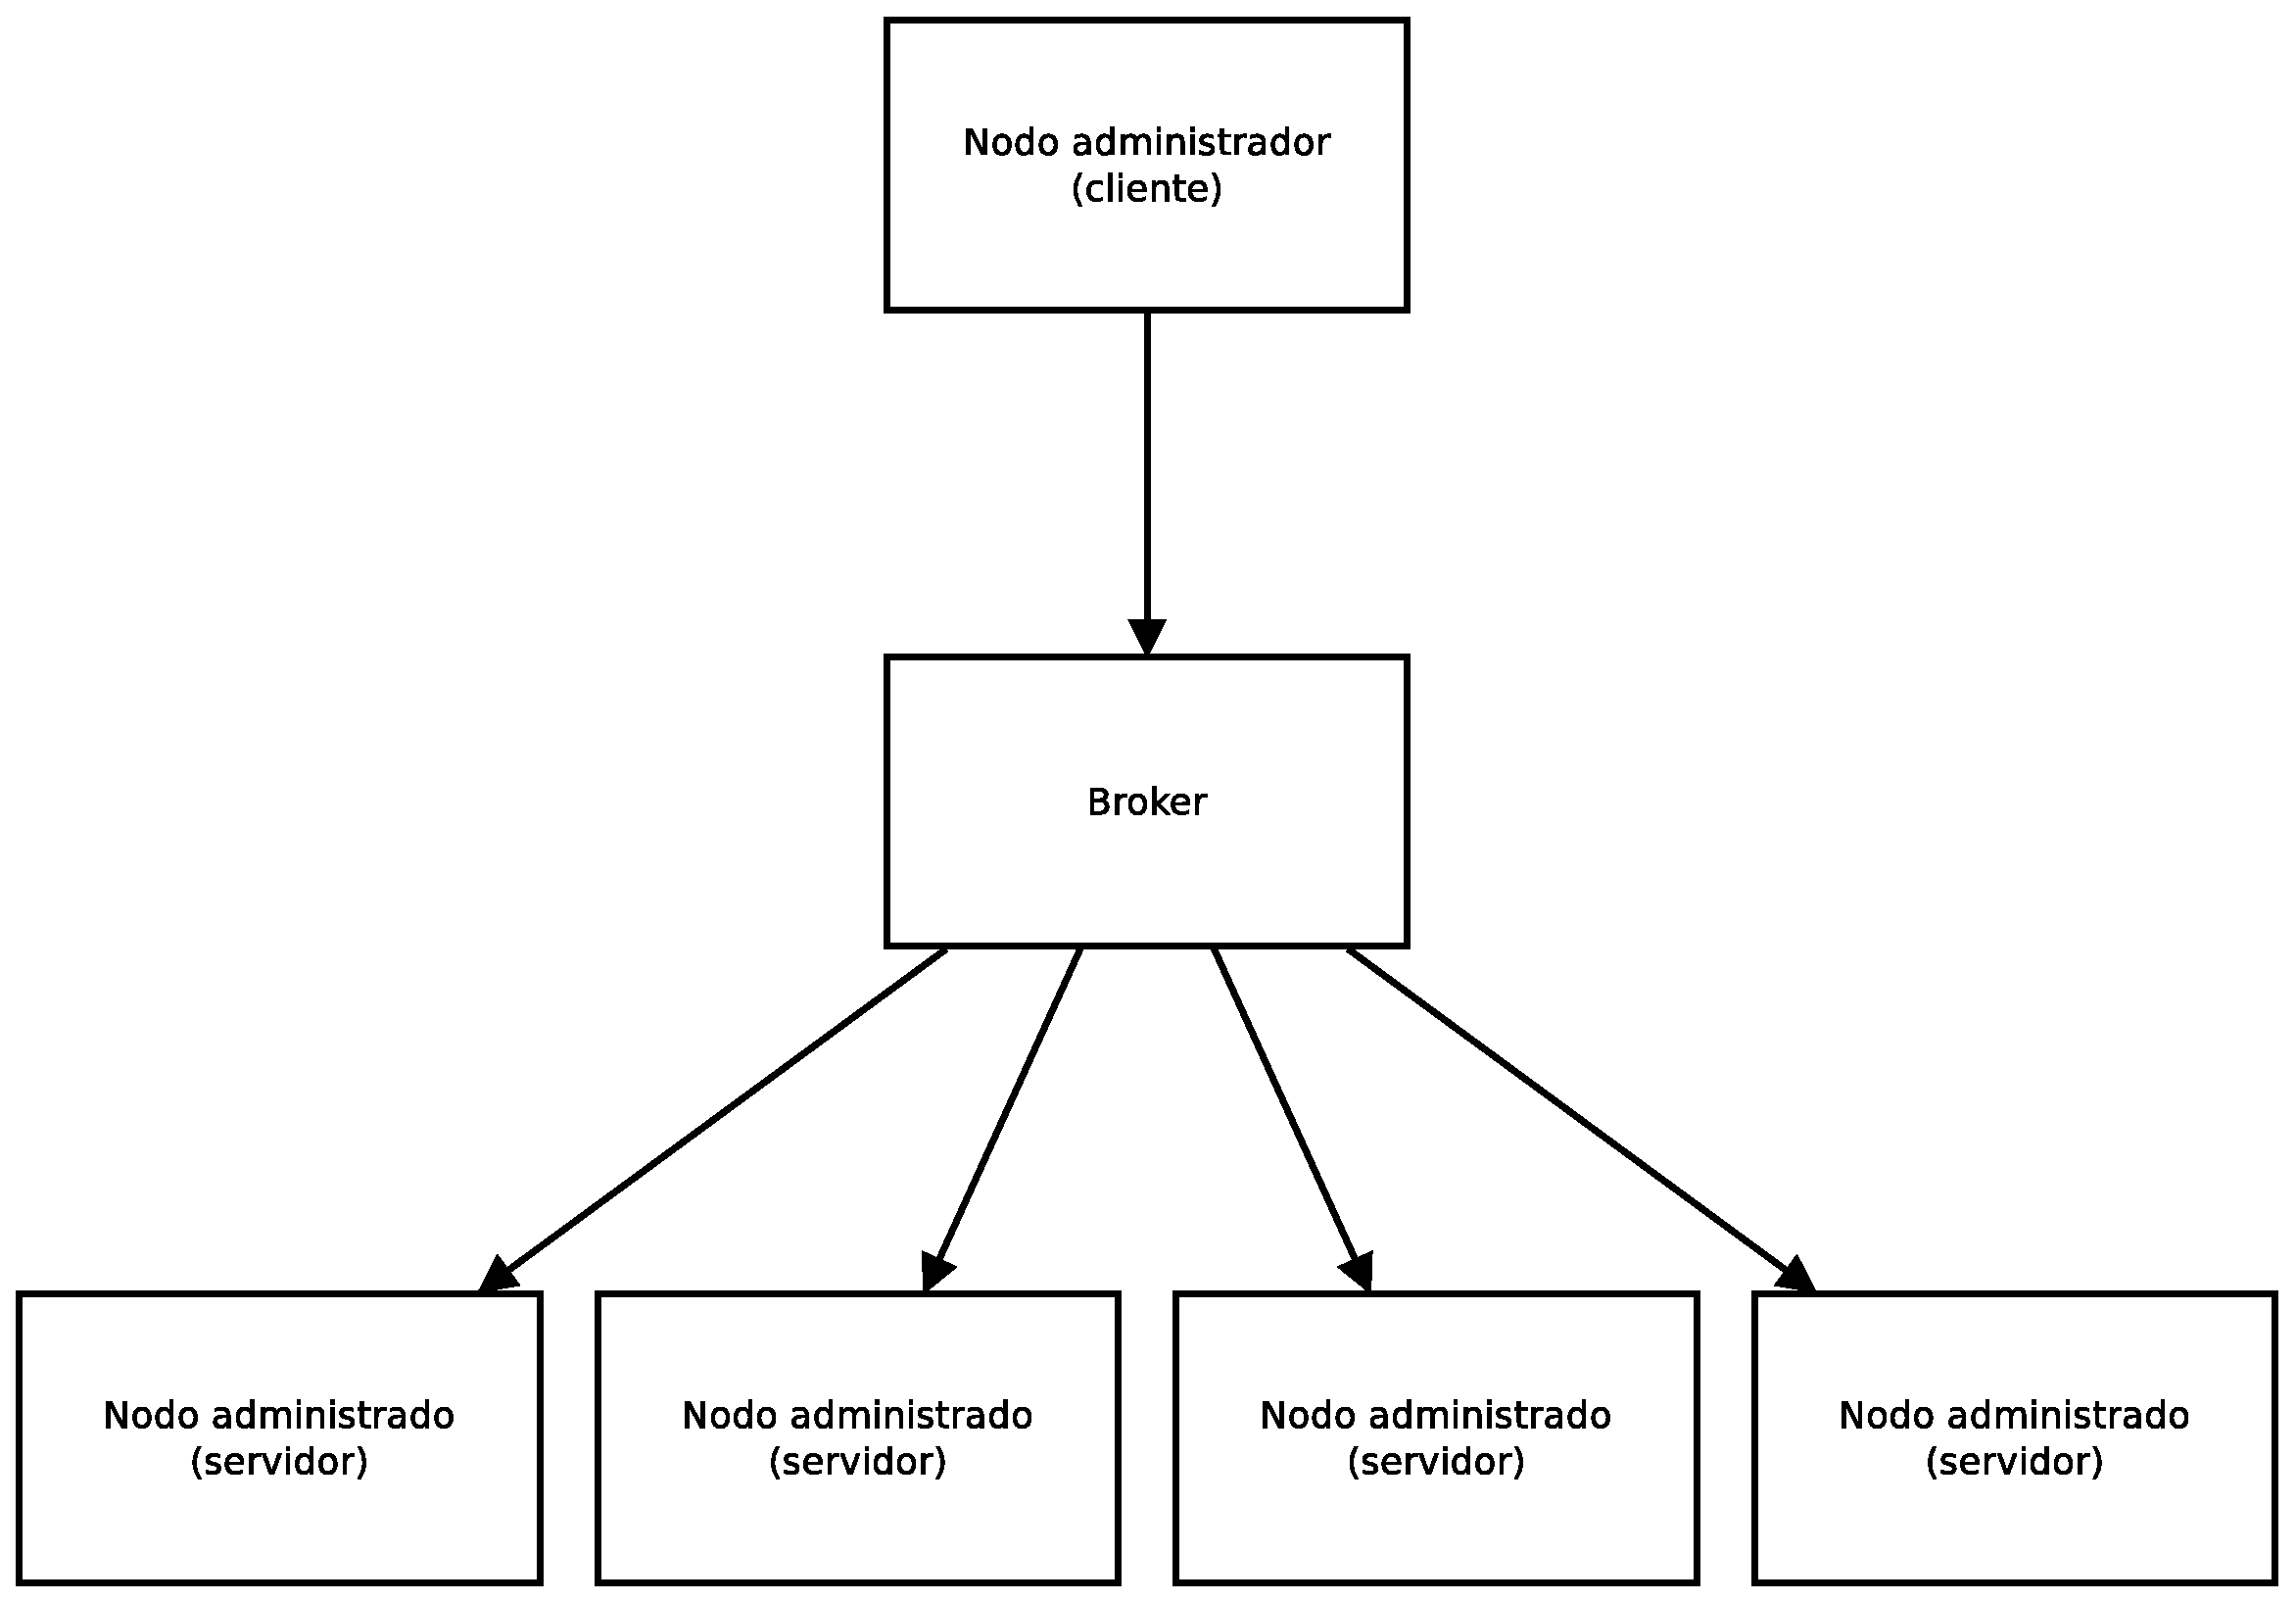
\includegraphics[width=13.5cm]{figuras/Arquitectura_MCollective.eps}
  \caption{Arquitectura de MCollective.}
\label{figure:arquitectura-mcollective}
\end{figure}

%%
\section{Instalación}

El primer paso consiste en la instalación de RubyGems. Para ello, consulta el apéndice \ref{comun:ruby} de instalación de Ruby y RubyGems.

Descargamos los paquetes \texttt{mcollective}, \texttt{mcollective-client} y \texttt{mcollective-common} de \url{http://downloads.puppetlabs.com/mcollective/}:

\begin{bashcode}
_: wget http://downloads.puppetlabs.com/mcollective/\
mcollective_1.2.1-1_all.deb
_: wget http://downloads.puppetlabs.com/mcollective/\
mcollective-client_1.2.1-1_all.deb
_: wget http://downloads.puppetlabs.com/mcollective/\
mcollective-common_1.2.1-1_all.deb
\end{bashcode}

Dependiendo de si el nodo va a ser administrador o administrado tendremos que instalar unos u otros paquetes:

\begin{tabular}{|c|c|c|}
   \hline
   Paquete & Nodo administrador & Nodo administrado \\ \hline
   mcollective-common & X & X \\ \hline
   mcollective-client & X &   \\ \hline
   mcollective &  & X \\ \hline
\end{tabular}
\\

Podemos instalar los paquetes de la siguiente manera:

\begin{bashcode}
_: dpkg -i mcollective*.deb
\end{bashcode}

Una vez instalado MCollective, instalamos la librería \texttt{libstomp-ruby}:

\begin{bashcode}
_: apt-get install libstomp-ruby
\end{bashcode}


%%
\section{Configuración}

A continuación hay que editar el fichero de configuración de MCollective. En los nodos administradores (clientes) se encuentra en \texttt{/etc/mcollective/client.cfg} mientras que en los nodos administrados (servidores) se encuentra en \texttt{/etc/mcollective/server.cfg}. Nos aseguramos de que contengan los siguientes valores:

\begin{bashcode}
plugin.stomp.host = 155.210.155.ABC # Direccion IP del MQ broker
plugin.stomp.port = 61613
plugin.stomp.user = mcollective
plugin.stomp.password = mcollective
\end{bashcode}


%%%%%%%%%%%%%%%%%%%%%%%%%%%%%%%%%%%%%%%%%%%%%%%%%%%%%%%%%%%%%%%%%%%%%%%%%%%%%%%%
\section{Comprobación de la instalación}

En el servidor stomp lanza el siguiente comando:

\begin{bashcode}
_: /usr/sbin/service rabbitmq-server start
\end{bashcode}

En los nodos administrados (servidores) lanza éste:

\begin{bashcode}
_: /usr/sbin/service mcollective start
\end{bashcode}

Y en uno de los nodos administradores (clientes) lanzaremos el comando \texttt{mc-ping}. La salida obtenida al ejecutar el comando debería ser similar a la siguiente:

\begin{bashcode}
_: mc-ping
155.210.155.177                       time=46.06 ms
---- ping statistics ----
1 replies max: 46.06 min: 46.06 avg: 46.06
\end{bashcode}


%%%%%%%%%%%%%%%%%%%%%%%%%%%%%%%%%%%%%%%%%%%%%%%%%%%%%%%%%%%%%%%%%%%%%%%%%%%%%%%%
\section{Versiones instaladas}

\begin{table}[!htbp]
\centering
   \begin{tabular}{|c|c|}
      \hline
      \textbf{Software} & \textbf{Versión} \\ \hline
      Ubuntu & 10.04 \\ \hline
      MCollective & 1.2.1-1 \\ \hline
      libstomp-ruby & 1.8 (1.0.4-1) \\ \hline
   \end{tabular}
\caption{Versiones instaladas de MCollective y libstomp.}
\label{table:mcollective-versions}
\end{table}
